\documentclass[11pt,spanish]{article}

% Paquetes
\usepackage{amstext}
\usepackage{amssymb}
\usepackage{babel}
    \addto\shorthandsspanish{\spanishdeactivate{~<>}}
    \decimalpoint
\usepackage{float}
\usepackage[T1]{fontenc}
\usepackage[a4paper]{geometry}
    \geometry{verbose,tmargin=3cm,bmargin=2cm,lmargin=2.5cm,rmargin=2.5cm}
\usepackage{graphicx}
\usepackage[utf8]{inputenc}
\usepackage{mathptmx}
\usepackage{units}

% tipo de fuente 
\usepackage{lmodern}

\makeatletter

\makeatother


\begin{document}

% Título
    \begin{center}
    \textsc{\large Física 2 (Física) - Cátedra Diana Skigin}
    \par\end{center}{\large \par}
    
    \begin{center}
    \textsc{\large Segundo Cuatrimestre de 2021}
    \par\end{center}{\large \par}
    
    \begin{center}
    \textsc{\large Guía 1: Oscilador Armónico Simple}
    \par\end{center}{\large \par}

% Comienzo 
\begin{enumerate}

% Ejercicio 1

    \item Escriba y resuelva las ecuaciones de movimiento asociadas con los
    siguientes sistemas: 

    \begin{enumerate}
        \item Péndulo de longitud $l$ en presencia de un campo gravitatorio con
        aceleración $g$. Discuta todas las aproximaciones que realiza.
        \item Oscilaciones longitudinales de una masa $m$ sujeta a dos paredes
        mediante dos resortes iguales de constante $k$, para los dos casos: 
    
        \begin{enumerate}
            \item longitud natural del resorte $l_{0}$ (con $ l_{0}<l$).
            \item \textit{slinky} (es decir, $l_{0}=0$). 
        \end{enumerate}
        
        \item Oscilaciones transversales del sistema del punto anterior,
        discutiendo las diferencias entre los casos i) y ii), y analizando 
        cuidadosamente las aproximaciones que realiza. En el caso i) analice
        la diferencia entre considerar que los resortes están tensionados en
        la posición de equilibrio $(l_{0}<l)$ o que están relajados en dicha
        posición $(l_{0}=l)$.
    
        \begin{figure}[H]
            \centering{}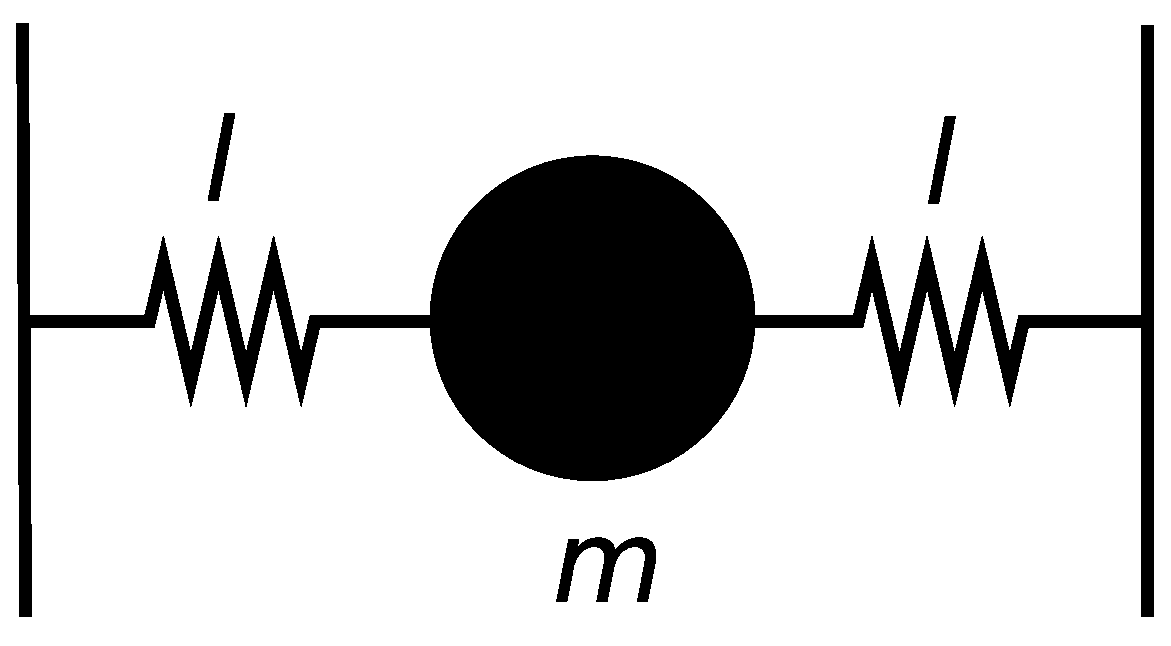
\includegraphics[clip,scale=0.25]{figs/ej1-1}
        \end{figure}
    
    \end{enumerate}


% Ejercicio 2

    \item Considere el movimiento de una masa $m$ sujeta a un resorte
    de constante elástica $k=m\omega_{0}^{2}$ y constante de
    amortiguamiento por unidad de masa $\Gamma$. Demuestre que el
    resultado para el oscilador ``sobreamortiguado'' dado por:
    \[
    x(t)=e^{-\Gamma t/2}\left\{ x(0)\cosh(\left|\omega\right|t) + \left[\dot{x}(0)+\frac{1}{2}\Gamma x(0)\right]\frac{\sinh(\left|\omega\right|t)}{\left|\omega\right|}\right\} 
    \]
    se deduce de las siguientes:
    \[
    x(t)=e^{-\Gamma t/2}\left\{ x(0)\cos(\omega t)+\left[\dot{x}(0)+\frac{1}{2}\Gamma x(0)\right]\frac{\sin(\omega t)}{\omega}\right\} 
    \]
    \[
    \omega=\pm i\left|\omega\right|,\,\,\,\left|\omega\right|=\sqrt{\frac{1}{4}\Gamma^{2}-\omega_{0}^{2}}
    \]
    \textbf{Sugerencia:} verifique primero las identidades $\cos(ix)=\cosh(x)$
    y $\sin(ix)=i\sinh(x)$; luego úselas.


% Ejercicio 3
    \item Comenzando con la ecuación general dada en el problema
    anterior para oscilaciones libres subamortiguadas, muestre que
    para amortiguamiento crítico la solucion es:
    \[
    x(t)=e^{-\Gamma t/2}\left\{ x(0)+\left[\dot{x}(0)+\frac{1}{2}\Gamma x(0)\right]t\right\} 
    \]
    Muestre que también se obtiene este resultado comenzando con la
    ecuación para oscilaciones sobreamortiguadas.

% Ejercicio 4
    \item 
    %\quad{}
    \begin{enumerate}
        \item Escriba la ecuación de movimiento para una masa $m$ sujeta a un
        resorte de constante elástica $k$ y constante de amortiguamiento por
        unidad de masa $\Gamma$, sobre la que se aplica una fuerza dependiente
        del tiempo $F(t)$. 

        \item Proponga la siguiente solución homogénea:
        $x_\text{h}(t)=Ce^{-t/2\tau}\cos(\omega_{1}t+\theta)$ y halle los
        valores de $\tau$ y de $\omega_{1}$. ¿De qué depende el valor de $C$ y
        de $\theta$? ¿Es lícito plantear las condiciones iniciales sobre la
        solución homogénea?
        
        \item Considere que $F(t)$ tiene la forma $F(t)=F_{0}\cos(\omega t)$ y
        proponga la siguiente solución particular:
        $x_\text{P}(t)=A\sin(\omega t)+B\cos(\omega t)$. Obtenga $A$ y $B$.
        Grafique cualitativamente $A$ y $B$ en función de $\omega$. Discuta si
        se pierde generalidad al suponer que la fuerza externa tiene esa forma.

        \item Grafique cualitativamente la posición de la masa en función del
        tiempo.

        \item Calcule la potencia media que se consume en el estado estacionario
        y la potencia media de pérdida por fricción. Verifique la igualdad
        de ambas potencias.
        
        \item Verifique que si $x_{1}(t)$ es solución de la ecuación diferencial
        cuando la fuerza externa es $F_{1}(t)$ y $x_{2}(t)$ lo es cuando
        la fuerza externa es $F_{2}(t)$, entonces $x(t)=x_{1}(t)+x_{2}(t)$
        será solución de la ecuación diferencial cuando la fuerza externa
        sea $F(t)=F_{1}(t)+F_{2}(t)$, si y sólo si las condiciones iniciales
        son la suma de las condiciones iniciales de los dos casos.
        
        \item Proponga ahora como solución particular la solución compleja
        $x_\text{p}(t)=Ae^{-i\omega t}$ y demuestre que
        $\mathfrak{Re}(A)=A_\text{elástico}$ y que
        $\mathfrak{Im}(A)=A_\text{absorbente}$. ¿Por qué es así?

    \end{enumerate}

% Ejercicio 5
    \item Sea un oscilador armónico con una frecuencia de oscilación
    $\nu_{0}=10\mbox{\,\ Hz}$ y con un tiempo de decaimiento muy largo. Si este
    oscilador es alimentado con una fuerza armónicamente oscilante y con una
    frecuencia de 10 Hz, adquirirá una gran amplitud, es decir, ``resonará'' en
    la frecuencia de excitación. Ninguna otra fuerza motriz oscilante en forma
    armónica producirá una gran amplitud (una resonancia). 

    \begin{enumerate}
        \item Justifique el enunciado anterior.

        \item Luego suponga que el oscilador está sujeto a una fuerza que es una
        pulsación cuadrada repetida periódicamente y cuya duración es $0.01$
        s repetida una vez por segundo. Describa cualitativamente el análisis de
        Fourier de la pulsación cuadrada repetitiva.

        \item ¿``Resonará'' el oscilador armónico (adquirirá una gran amplitud)
        bajo la influencia de esta fuerza motriz?
 
        \item Suponga que la fuerza motriz es la misma pulsación cuadrada (de
        ancho $0.01$ s) pero repetida dos veces por segundo. ¿Resonará el
        oscilador? Responder a la misma pregunta para velocidades de repetición
        de 3 a 9 segundos.
    \end{enumerate}

\end{enumerate}

\end{document}
